% CS 217A/B, Winter/Spring 2017
% Professor Lixia Zhang
% Project Final Report

\documentclass{sig-alternate}

% General packages and setup
\PassOptionsToPackage{hyphens}{url}\usepackage{hyperref}  % For embedding clickable links to citations
\paperheight=11in
\renewcommand\_{\textunderscore\allowbreak}  % Allows line breaks on words with underscores

% Begin packages/setup for timeline
%\usepackage[utf8]{inputenc}
%\usepackage[TS1,T1]{fontenc}
%\usepackage{fourier, heuristica}
%\usepackage{array, booktabs}
%\usepackage{graphicx}
%\usepackage[x11names]{xcolor}
%\usepackage{colortbl}
%\usepackage{caption}
%\usepackage{tikz}  % checkmark icon
%\usepackage{wrapfig}
%\usepackage{soul}  % strikethrough
%
%\DeclareCaptionFont{blue}{\color{LightSteelBlue3}}
%\newcommand{\foo}{\color{LightSteelBlue3}\makebox[0pt]{\textbullet}\hskip-0.5pt\vrule width 1pt\hspace{\labelsep}}
%\def\checkmark{\tikz\fill[scale=0.4](0,.35) -- (.25,0) -- (1,.7) -- (.25,.15) -- cycle;}	% Checkmark icon
% End packages/setup for timeline

\begin{document}
	
\title{ndnMouse\\Secure Control Interface for a PC Using a Mobile Device}
\subtitle{CS 217B Project Final Report, Spring 2017}
\numberofauthors{1}
\author{
	Wesley Minner\\
	Computer Science M.S. Student\\
	wesleyminner@gmail.com
}

\date{18 May 2017}
\maketitle

% ==============================================================================
\begin{abstract}
This report outlines the results of my efforts on ndnMouse, my class project for CS 217B, as well as my Master's Capstone project. It is open-sourced on \href{https://github.com/wminner/ndnMouse}{Github} under the GNU public license, and available on the \href{https://play.google.com/store/apps/details?id=edu.ucla.cs.ndnmouse}{Google Play App Store}. The goal of ndnMouse is to securely and efficiently control one or more personal computers via remote mouse movement and rudimentary keyboard commands from your phone, running the communication protocol over Named Data Networking (NDN)~\cite{ndn}. In order to compare the design and performance benefits of NDN, ndnMouse also supports communication over UDP. Implementation of both protocols resulted in fairly unique server and clients designs. The pros and cons of each will be explored in this report.

Section 1 will review the features and use cases of ndnMouse, with more detail of the command protocol in Section 2. Details on the security features will be given in section 3, with challenges and trade-offs I have overcome listed in section 4. Performance analysis comparing NDN and UDP implementations is in section 5. Finally section 6 explores extensions and future use cases for ndnMouse. Additionally screenshots of the application are in section 7, the Appendix.
\end{abstract}

\keywords{NDN, Mouse, Keyboard, Remote Access, Security}

% ==============================================================================
\section{Overview}
NdnMouse provides remote access to the mouse and keyboard of a PC in order to provide a simple and convenient way to wirelessly interface with your computer. The main use case was to support wireless slideshow/powerpoint control, removing the need for a proprietary piece of hardware (such as a USB clicker device). Anecdotal evidence suggests that users of these devices encounter a variety of issues such as: drained batteries, poor connection, and general hardware failure. Additionally a presenter must also carry around the clicker hardware, which has no other than slideshow control. NdnMouse removes the need for a specialized clicker and adds remote slideshow control to something most people already carry around in their pockets, a smart phone. 

By taking advantage of the local WiFi access point or the phone's WiFi hotspot feature, a user can use their Android smart phone as a virtual touchpad and simple keyboard, providing the functionality needed to step through a powerpoint presentation without any additional hardware. NdnMouse also may be of use during times of hardware failure, providing an emergency backup mouse or keyboard when the user has limited options to interface with their PC.

Both NDN and UDP/IP transport/routing protocols are supported, encrypting packets with AES if a password is provided by the user. Additionally NDN can provide some extra features in the form of interest (query) condensing, allowing the phone server to better scale its performance when multiple PC clients are connected. More on this idea will be described in Section 5. However the protocol choice should ideally be transparent to the user, as all features are supported on both NDN and UDP.

\subsection{Features}
NdnMouse supports full mouse control: relative cursor movement, left click, right click, and a shortcut allowing tap-to-click on the touchpad. Sensitivity and precision settings are also provided, for fine tuning the feel of the movement. Two-finger scrolling works similarly to Apple laptops, with inversion and sensitivity settings as well. Rudimentary keyboard support allows the user to execute common slideshow control commands, such as using the arrow keys or the spacebar to easily change slides. Additionally custom typed messages are supported, allowing the user to type any message using the built-in Android keyboard. Upon sending the message, all receiving client PCs will then virtually the characters out instantly on whatever program window is selected at that time.

The security for ndnMouse was designed to defend against packet snooping, replay attacks, privacy attacks, and brute force attacks. More details will be given in section 3. The user may also choose to not use a password, which sends the communication protocol in cleartext and avoids a minor amount of encryption/decryption overhead. 

\subsection{Supported Platforms}
NdnMouse is composed of two applications: the server/producer Java application (running on the Android phone), and the client/consumer Python application (running on the PC). Any relatively modern Android phone is supported (Android 4.1 and up), and basically any PC that can run NDN's Network Forwarding Daemon (NFD)~\cite{nfd} and Python3~\cite{python3}. Since Python runs on the three major operating systems (Linux, OSX, and Windows), the limiting factor is NFD, which only currently runs on Linux and OSX. However Windows PCs can still use ndnMouse by limiting their protocol choice to UDP only.

Other dependencies include a few Python libraries needed for the PC client, specifically PyAutoGUI~\cite{pyautogui}, PyCrypto~\cite{pycrypto}, and PyNDN~\cite{pyndn}. PyAutoGUI provides mouse and keyboard control, as well as some simple dialog boxes for collecting user input. PyCrypto handles all the cryptography operations, and PyNDN provides the API for using NDN and for interfacing with NFD. The Android application uses jNDN~\cite{jndn} to access the NDN API, but this library comes compiled into ndnMouse's APK and requires no outside installation by the user. Both the PC and Android phone must have NFD installed and running to communicate over NDN.

\section{Protocol}
NdnMouse can run its communication protocol four different ways, depending on the transport protocol used (UDP or NDN) and if a password is provided by the user (security on or off).

\subsection{UDP}
Without a password (all security off), packets are transmitted in cleartext and are at most 16 bytes. UDP uses connection-oriented communication by having the client send an \texttt{OPEN} message to the server, similar to a TCP \texttt{SYN} packet. This asks the server to establish a \textit{session} between the client and itself. An \texttt{OPEN-ACK} reply message is used to respond to the \texttt{OPEN} message and completes the connection setup.

Once a session is established, the server will send unsolicited mouse commands\footnote{I will refer to all commands ndnMouse can send as mouse commands, though this includes supported keyboard commands as well.} to its clients. The data format is not strict across all possible mouse commands, but generally takes the form of one character dictating the type of command, followed by any additional information for that command. For example, a mouse movement command is of the form \texttt{M<x-4B><y-4B>}. I denote the \textit{x} and \textit{y} coordinates each have a fixed length of 4 bytes by appending "\texttt{4B}." See \hyperlink{tab:msgFormat}{Table 1} for the supported, non-secure message formats.

\begin{table}
	\hypertarget{tab:msgFormat}{}
	\begin{center}
		\begin{tabular}{| l | l |}
			\hline
			Message Type & Message Format\\ \hline\hline
			Movement & \texttt{M<x-4B><y-4B>}\\ \hline
			Click & \texttt{C<click\_message>}\\ \hline
			Scroll & \texttt{S<x-4B><y-4B>}\\ \hline
			Keyboard & \texttt{K<keyboard\_message>}\\ \hline
			Typestring & \texttt{T<type\_string-10B-max>}\\ \hline
		\end{tabular}
		\caption{Non-secure message formats}
	\end{center}
\end{table}

Heartbeat messages are sent once every one second to keep the connection alive when no other mouse command packets are being sent. The client query packet contains the message \texttt{HEART}, and the server reply contains the message \texttt{BEAT}. The main goal of heartbeats was to detect when the server had lost its session with the client, such as during a server reset or crash. In these cases, the client would miss a certain number of heartbeat replies from the server, triggering a session restart on the client side. The client would then try to open a new session using \texttt{OPEN} messages. After receiving a \texttt{OPEN-ACK}, the session would resume normal activity.

Lastly a \texttt{CLOSE} message is sent by the client upon exiting the application. This lets the server know that it can stop sending unsolicited mouse command messages 


\begin{table}
	\hypertarget{tab:secureMsgFormat}{}
	\begin{center}
		\begin{tabular}{| l | l |}
			\hline
			Message Type & Secure Message Format\\ \hline\hline
			Movement & \texttt{<seq-4B>M<x-4B><y-4B>}\\ \hline
			Click & \texttt{<seq-4B>C<click\_message>}\\ \hline
			Scroll & \texttt{<seq-4B>S<x-4B><y-4B>}\\ \hline
			Keyboard & \texttt{<seq-4B>K<keyboard\_message>}\\ \hline
			Typestring & \texttt{<seq-4B>T<type\_string-10B-max>}\\ \hline
		\end{tabular}
		\caption{Secure message formats}
	\end{center}
\end{table}

\subsection{NDN}

%My application runs a custom, connectionless protocol (for both UDP and NDN implementations) that passes simple man-readable (when unencrypted) mouse control commands in the form of 48 byte packets (when using security). The protocol is not optimal regarding the encoding of commands. However the man-readable nature of the commands has made debugging considerably easier during development. I may consider re-designing the protocol when I know the entire command set that the app will need to handle.  However at most, I can save 16 bytes off of each packet (lowering the total packet size to 32 bytes). This is due to the requirements of AES~\cite{cipher} cipher block chaining (CBC), which supports key lengths of 128, 192, and 256 bits. I am using a 128 bit (16 byte) key from the hashed user-password, so the total packet length must always be a multiple of 16 bytes. A 16 byte, random, cleartext initialization vector (IV) must also be included in each packet to ensure that two packets with the same cleartext content never encrypt to the same ciphertext. A 16 byte IV and a 16 byte message results in a minimum packet size of 32 bytes. I may consider using another style of AES encryption (like electronic codebook) if I am able to reduce the packet size considerably later in the project.

\subsection{Mouse Packets}

% ==============================================================================
\section{Security}

\subsection{Encryption}

\subsection{Password Salting}

\subsection{Sequence Number Validation}

\subsection{Attack Types and Defenses}
	
% ==============================================================================
\section{Challenges and Trade-offs}

\subsection{Signature Validation vs Shared Secret}


%\subsection{Unsolicited Data}
%UDP can easily send unsolicited data through a socket, but NDN cannot send unsolicited data through a face. By design, it must receive an interest packet first. For my application, unsolicited data is useful to send unpredictable mouse commands, like mouse clicks, avoiding the need for continuous polling from the client side. Mouse movement, on the other hand, must be continuously polled at a constant rate, which translates nicely to the NDN interest/data model.
%
%To handle mouse clicks using NDN, I created a separate interest that would ask the producer for mouse click data at a constant rate. A majority of the packets time out due to no available data, but when the user does execute a mouse click, the consumer side will still receive the mouse click data in a timely manner. Though this method is not as efficient as UDP, the latency is still low enough to be imperceptible by the user.
%
%\subsection{Encryption}
%Much of my protocol's design came from lessons learned during the implementation of UDP encryption. In order to support a connectionless session between server and client, I needed to ensure that each packet could be decrypted without any additional shared state between the server and client. This led me to the idea of attaching the appropriate cleartext IV to each packet, necessary to perform the decryption.
%
%The threat of inter-session replay attacks became another major design influencer, which required me to use some sort of shared state to let the client/server know that a packet was old (potentially replayed) and should be discarded. To accomplish this, a sequence number was prepended to each mouse command before encryption occurred. Therefore it would not be visible to any malicious users, and the client/server could toss any incoming packets that used an old sequence number. 
%
%While this solution prevents replaying packets during any particular session of ndnMouse, it does not prevent malicious users from successfully replaying packets \textit{across} sessions (assuming the ndnMouse user typically uses the same password each session). This is because the sequence number resets each time a new session is started, so \textit{once-old} packets from a previous session will become \textit{new} packets when a new session is started. This problem can be solved by using a shared, random, password salt to alter the key used for encryption each session. I have not yet implemented this behavior, but it is on my to-do list.


% ==============================================================================
\section{Performance Analysis}

\subsection{UDP vs NDN}

\subsection{Event Driven Architecture}

\subsection{Stateful Multi-Threaded Architecture}

% ==============================================================================
%\section{Expectations}
%My expectations have only slightly changed since my initial project proposal. I plan to focus on the security aspects of NDN, implementing full mouse control with some basic keyboard control (to support remote slide show/powerpoint control). During my security implementation work, I realized that the signature validation capabilities of NDN may not be practical for ndnMouse's purposes. Requiring the user to install certificates and a trust anchor ahead of time for each of their devices is significantly more work than using a simple user-password. Using asymmetric encryption via certificates to securely pass a symmetric encryption key between devices also adds an unneeded extra step to each session setup, which I currently skip by requesting a offline, shared secret from the user in the form of a password. For these reasons I will deprecate the signature validation requirements for ndnMouse and focus on other quality of life enhancements for the user. I may return to signature validation experimentation if I have extra time at the end of the quarter.
%
%I am slightly ahead of my initial timeline projections, but I also plan to finish somewhat early to gain the Capstone faculty signatures required for graduation. If all goes well, there may be at least one week I can use to add additional ease-of-use features, such as two-finger scrolling support. For now I am focusing on the minimum viable product, which includes mouse control, basic keyboard support, and full encryption security.


% ==============================================================================
% Bibliography
\bibliographystyle{abbrv}
\bibliography{sigproc}  % sigproc.bib is the name of the Bibliography in this case

% ==============================================================================
\section{Appendix}
Screenshots of the Android and PC applications follow. The Android app can be downloaded directly from the \href{https://play.google.com/store/apps/details?id=edu.ucla.cs.ndnmouse}{Google Play App Store}, and the PC client application can be downloaded from the \href{https://github.com/wminner/ndnMouse/tree/master/pc_client}{Github} repository.

\begin{figure}[ht]
	\hypertarget{fig:start}{}
	\centering
	\caption{Start screen}
	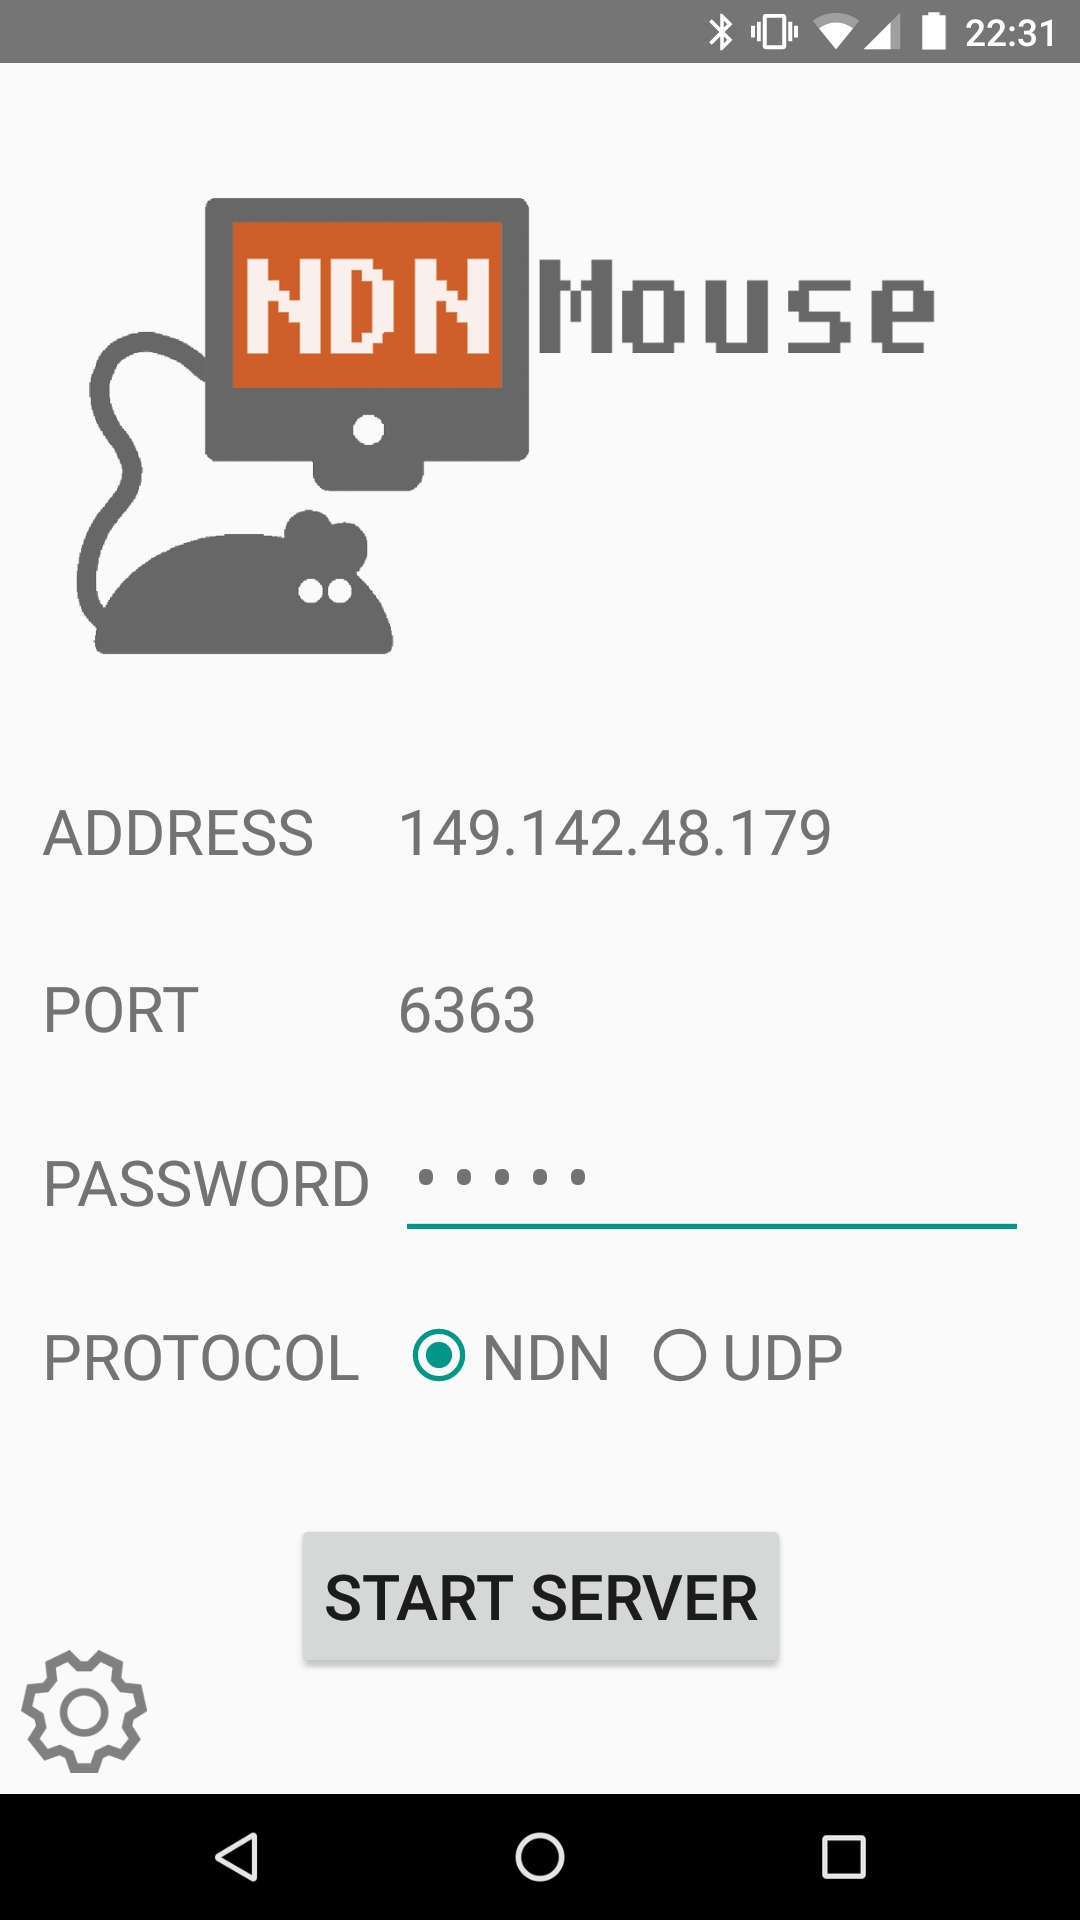
\includegraphics[width=6cm]{screenshots/start}
\end{figure}

\begin{figure}[ht]
	\hypertarget{fig:settings}{}
	\centering
	\caption{Settings screen}
	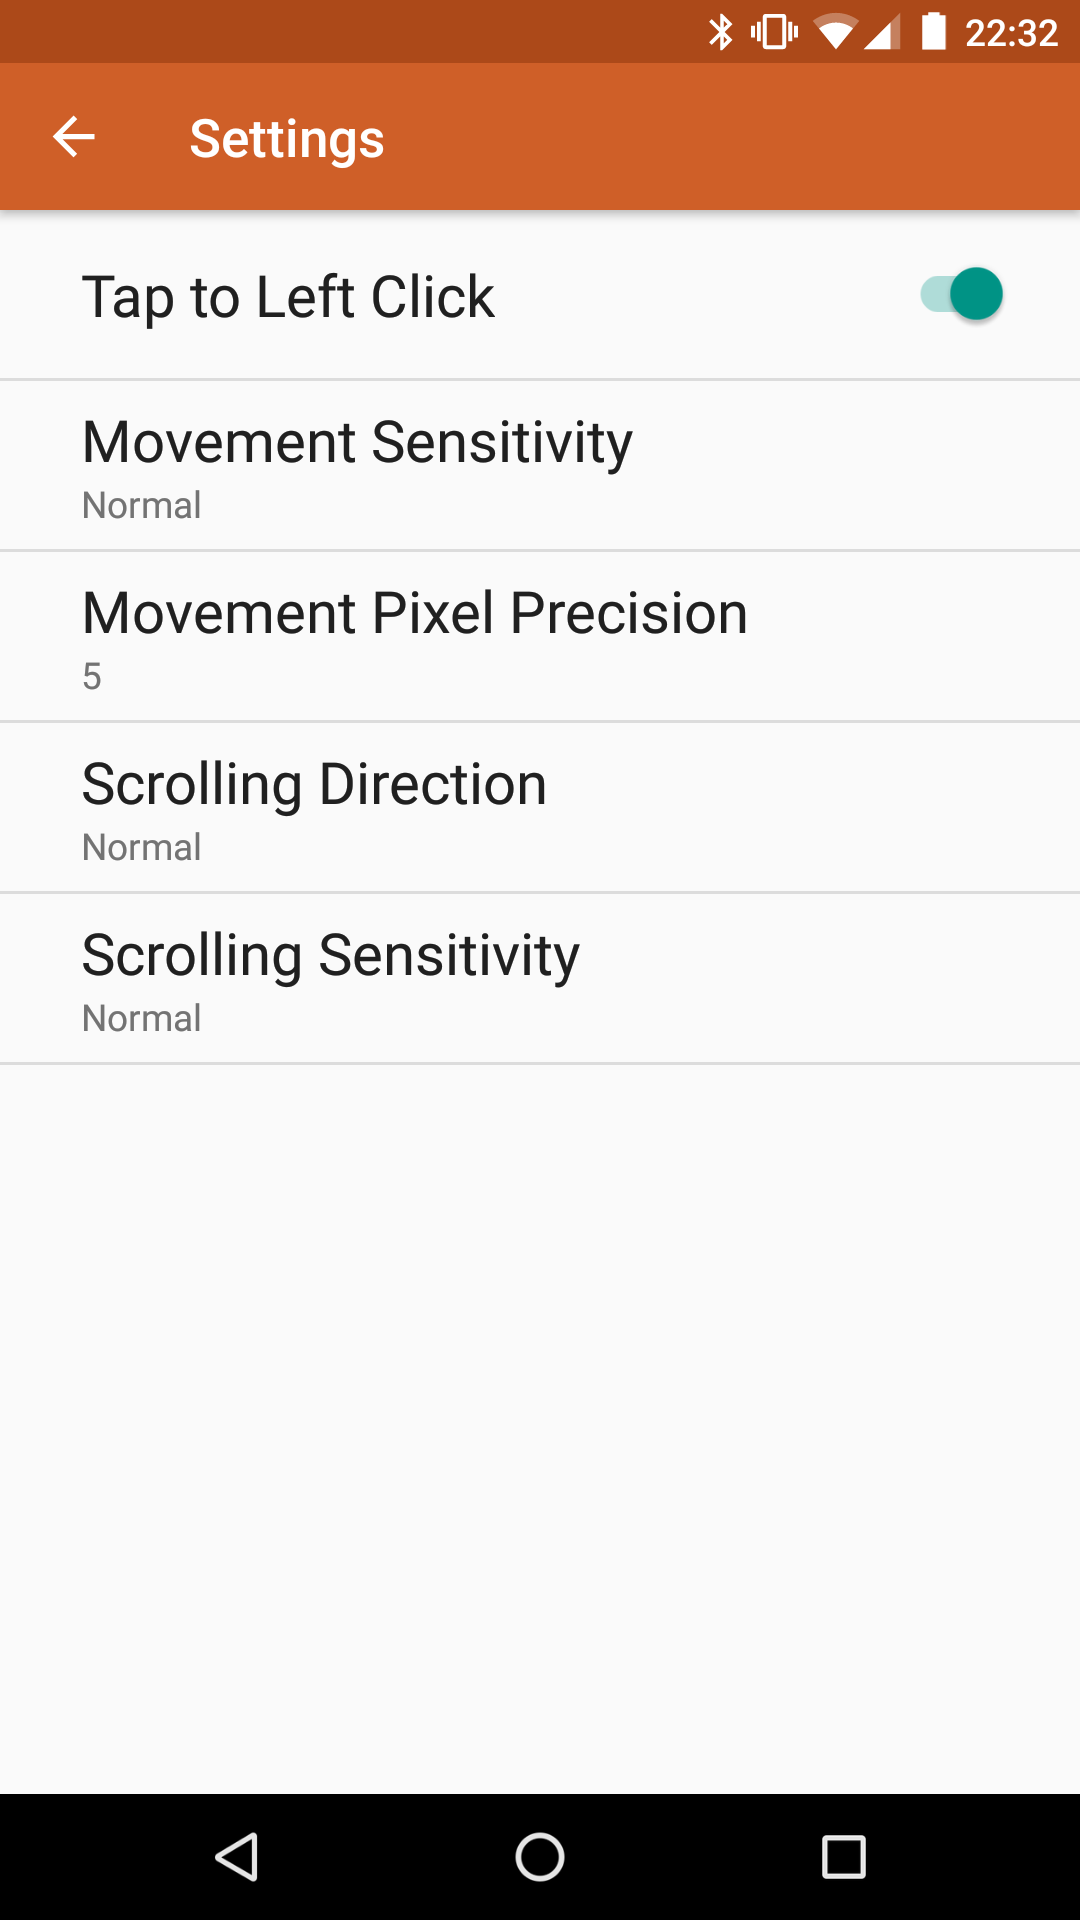
\includegraphics[width=6cm]{screenshots/settings}
\end{figure}

\begin{figure}[ht]
	\hypertarget{fig:touchpad}{}
	\centering
	\caption{Touchpad screen}
	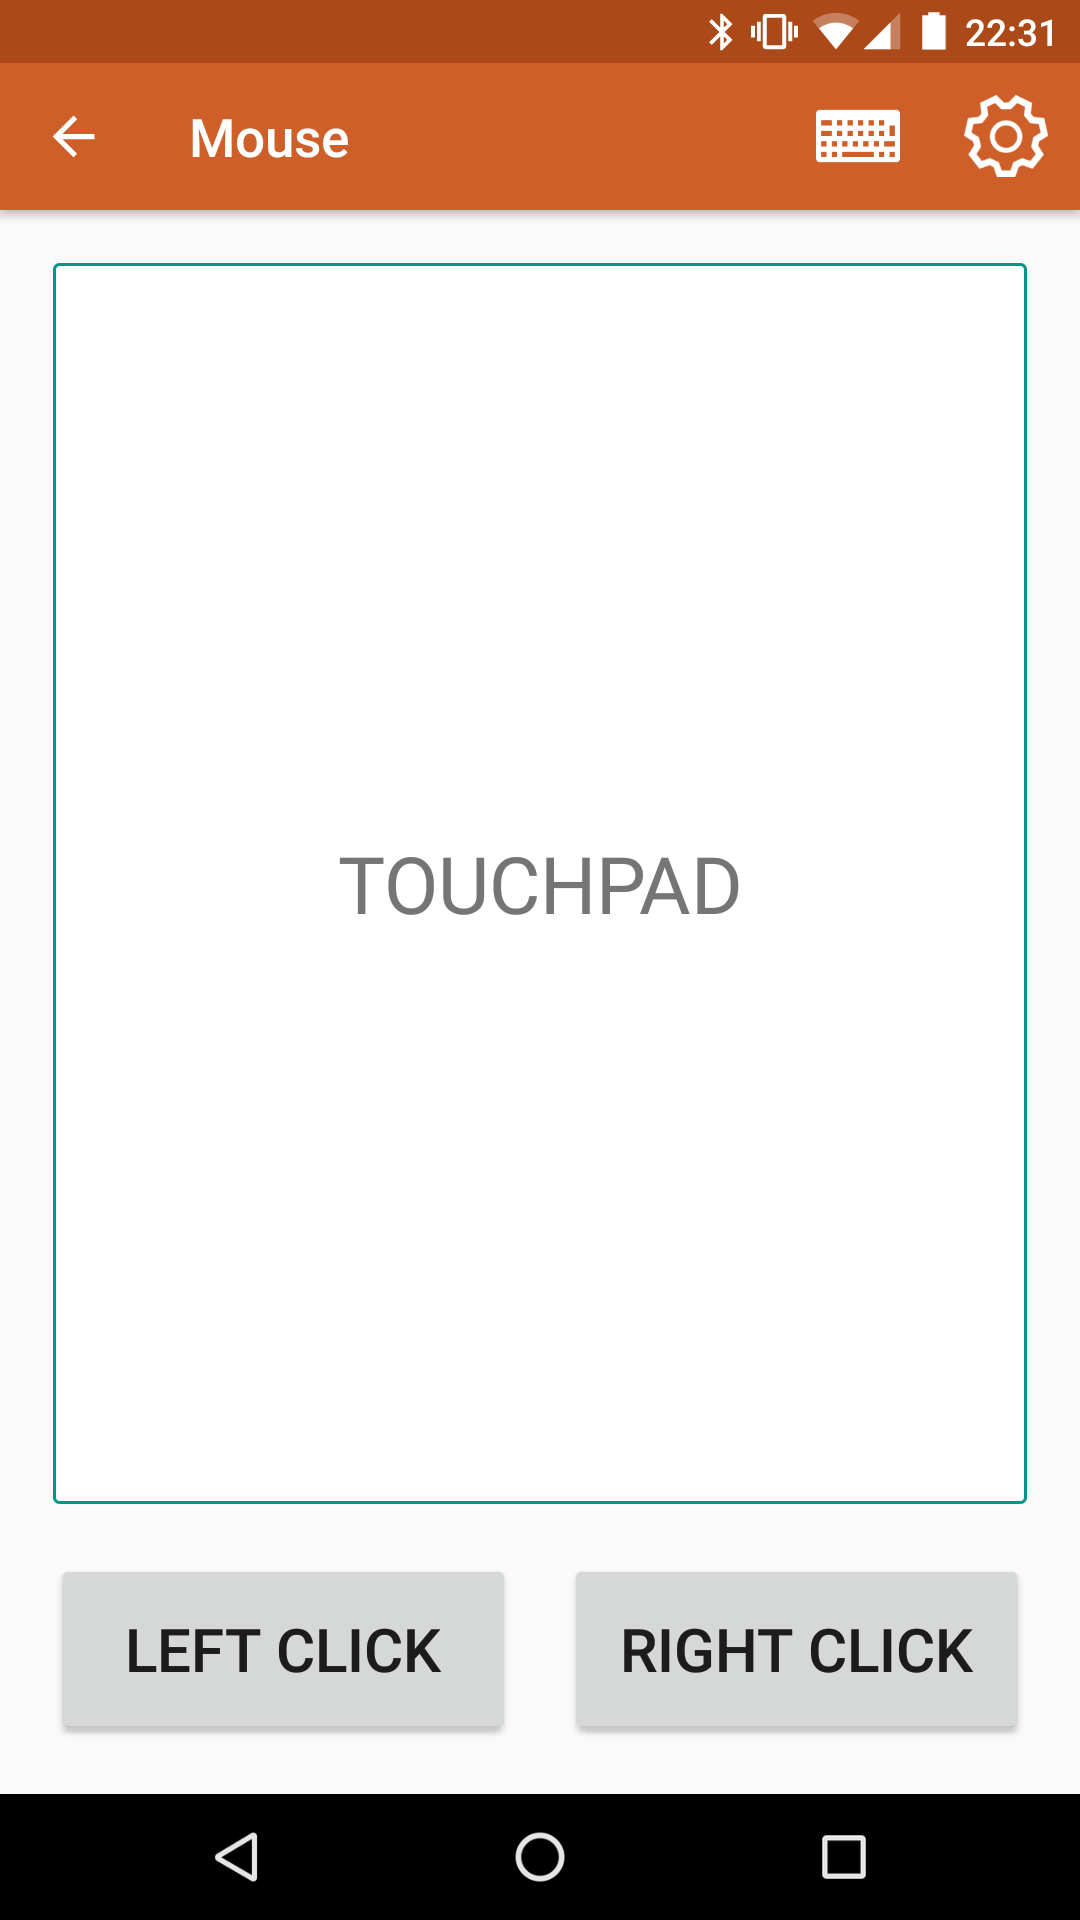
\includegraphics[width=6cm]{screenshots/touchpad}
\end{figure}

\begin{figure}[ht]
	\hypertarget{fig:keyboard}{}
	\centering
	\caption{Keyboard screen}
	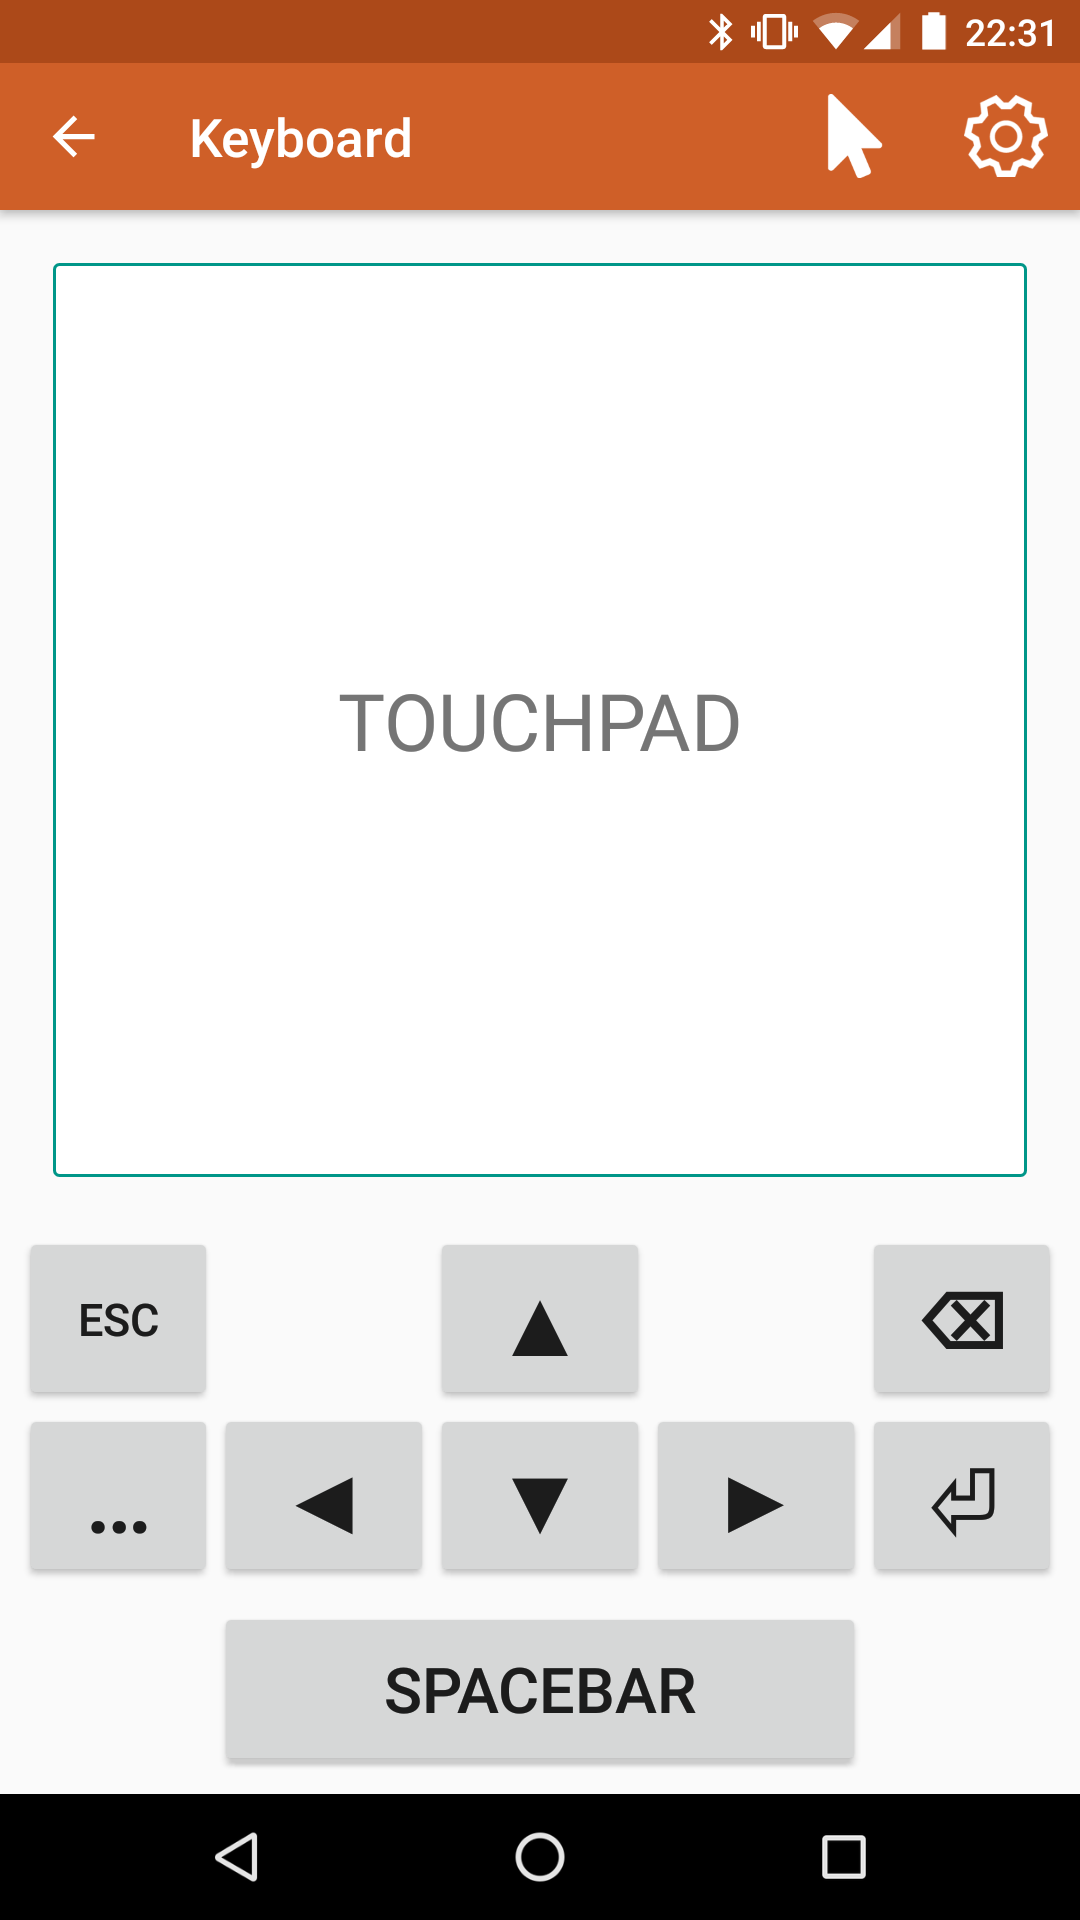
\includegraphics[width=6cm]{screenshots/keyboard}
\end{figure}

\begin{figure}[ht]
	\hypertarget{fig:custom\_type\_message}{}
	\centering
	\caption{Custom typed message entry}
	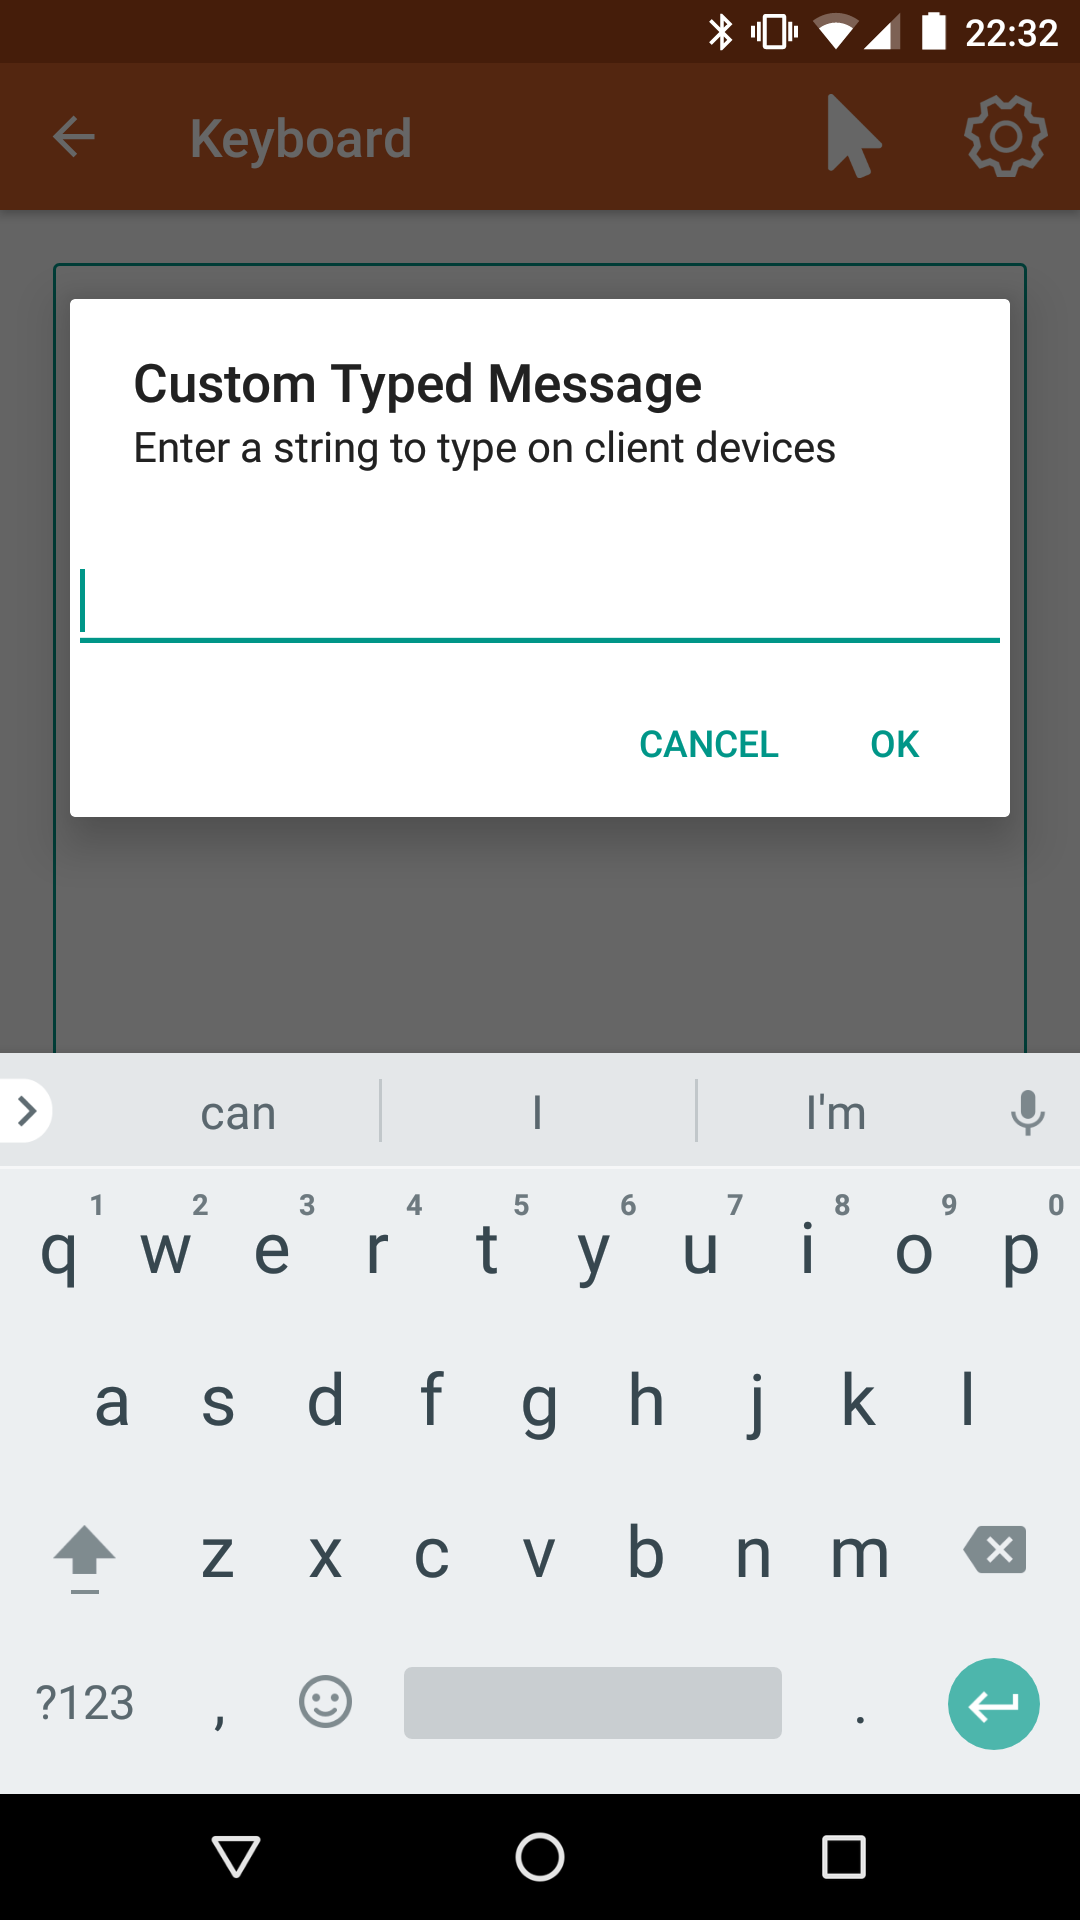
\includegraphics[width=6cm]{screenshots/custom_type_message}
\end{figure}

\begin{figure}[ht]
	\hypertarget{fig:client1}{}
	\centering
	\caption{PC program IP address entry}
	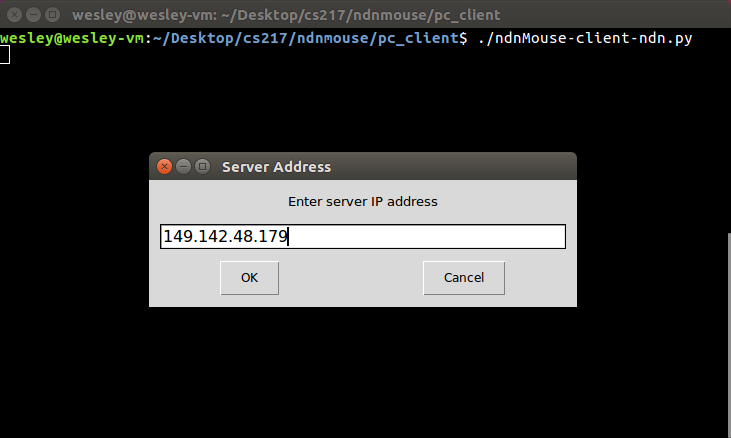
\includegraphics[width=11cm]{screenshots/client1}
\end{figure}

\begin{figure}[ht]
	\hypertarget{fig:client2}{}
	\centering
	\caption{PC program password entry}
	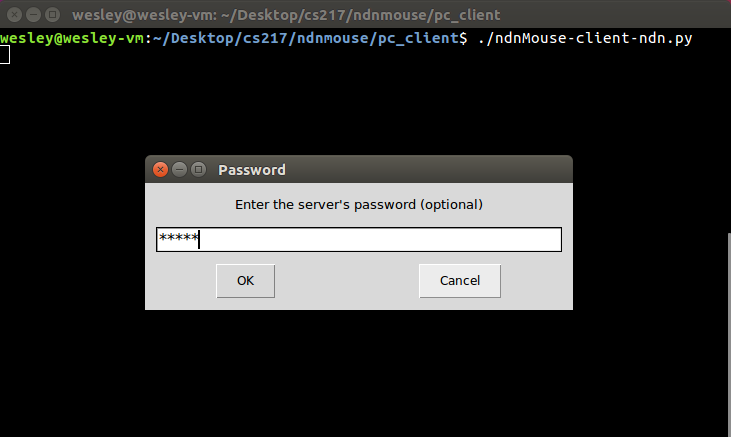
\includegraphics[width=11cm]{screenshots/client2}
\end{figure}

\begin{figure}[ht]
	\hypertarget{fig:client3}{}
	\centering
	\caption{PC program running}
	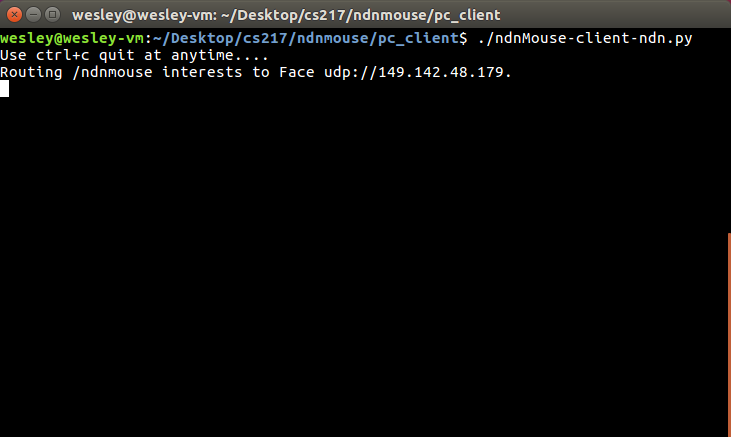
\includegraphics[width=11cm]{screenshots/client3}
\end{figure}

\end{document}